% vim: spelllang=en spell textwidth=120
\documentclass[deska]{subfiles}
\begin{document}

\chapter{Server part of deska}
\label{sec:deska-server}

\begin{abstract}
Talk about server part of deska application. Deska server application and deska database.
\end{abstract}

\section{Server and its database}
Server part of deska application can be devided into two parts. The {\em deska-server} and {\em deska-database}.
Deska-server is python application, that runs for every user, listen for the commands from deska-cli (see dbapi protocol).
Main work is to load json data, call corresponding stored function, and return the answer to deska-cli.
There are some special functions (freezeChangeset, showConfigDiff etc.) that are not implemented by deska db, but the server itselfs.

\section{Deska-server}
FIXME: about deska server configuration generators & some tricks (maybe) in deska-server to explain.

\section{Deska-database}
Deska-database is Postgresql database server, storing all data of user given schema, its relations and all changes of data.
There are tables, specified by user before build deska-database, tables for history tracking and many function for data manupulation.

\subsection{Data storage}
To prevent misunderstanding, if we talk about database, we use word {\em schema} in two different meanings. {\em User defined schema},
with meaning tables, with constraints describing data, that user wants to store into database. And {\em schema}, term used by
postegresql with meaning something as namespace containing database objects (tables, types, functions etc).
It is similar to Oracle's package. If we talk about user defined schema, we write the whole term, and if we talk about schema, we write
schema plus its name.

Lets look at how data are stored in deska database. Three types of data are stored in deska-database.

At first, there are information
about user defined database schema. These information are provided by {\tt kindNames}, {\tt kindAttributes} and {\tt kindRelations} functions.
Althouhg of many these information can be read from database catalog, there are stored in {\tt generated.py} file, which is used by
functions listed above, to get asked information. This kind of implementation, does not need access to database catalog or any table.

Second, the why we are here - the meaning of life, user data, fitting into user defined schema.
Objects and its attributes are stored in tables. 
After changeset is started, all data stored into database, are place into tables in history schema. Every kind has table in history
schema, with all attributes defined in user defined schema, and some more for history tracking.
There are tables defined by user, stored in schema production. These tables
(with its constraints) are used for validate data when commiting changeset, if data are successfully copied into tables in schema production,
from tables in schema history data are valid, corresponding to user defined schema.
FIXME: for more info see...

Third, there has to be some information about revisions and changeset. There are two tables, version (the name was here before
we start using {\em revision}) and changeset, for storing information about revisions and changeset. These tables are
in versioning schema.

\subsection{Data manipulation}
For manipulation with stored data, there is many stored procedures, in postgresql called {\em functions}.
Every action on data, as create object, set attribute, delete object, get object data, create changeset, delete changeset etc.,
has a function that do that. For object and its attributes, there are in genproc schema and are generated by
FIXME: how we call generator this exactly?
For changesets and versions, there are written by hand, and stored in deska schema, with many helping functions.

\subsection{Comunication}
All comunication with deska-server is implemented in schema json. There are functions, written in pgpython, which use another
functions, to manipulate with data in database. Or get data directly from tables as in {\tt pendingChangeset} and {\tt listRevisions}.
Why we created this layer, and why it returns json data and not table or normal value, will be described in section Json schema.
FIXME: link

\subsection{Json schema}
After we have generated functions for manipulating with data, and DBAPI specified, it was clear, that there must be some layer,
that transforms createObject(kindName,xxx) to kindName\_add(xxx), which is call of generated sql function.
We do that in deska-database, because we wanted to have 1:1 mapping between database functions, and DBAPI commands.

It works well until first performance testing was made. The state was, that deska-server call for data - milions of objects,
database worked and worked and... when finally returned this data to server, server started transformation... It takes long time
and consumes lots of memmory.
In the same time, diffing implementation started, and there where problems with many functions of different result types,
that has to be called, which was hard to union into one function.
So there was an idea, that json can be created inside database, so that the union of diffing function can return json.

Some test were run, the time for smaller data was worse with json in database, but for large data, there was significant
speed up.
FIXME: get results of these tests

The result is, that every function callable by server returns json.

\subsection{Getting data from tables}
Here we talk about getting data of objects, revisions and changesets stored in tables.
There are {\tt pendingChangeset} that selects data from changeset table, and {\tt listRevisions} that selects data from version table.
Both accept filter as parameter and uses some cast optimalization, about which we will talk in section cast optimazation.
FIXME: link

Object data functions {\tt objectData}. {\tt resolvedObjectData}. {\tt resolvedObjectDataWithOrigin} calls generated functions 
that returns tuple of attribute values, that is just converted into json format and returned. 

Functions {\tt multipleObjectData}. {\tt multipleResolvedObjectData} and {\tt multipleResolvedObjectDataWithOrigin} has parameter revision.
Postgresql does not have parametrized view, so we have to use function, to implement it. How this fact complicates filtering will
be described in section FIXME:link filtering issue.

\subsection{Db schemas}
FIXME: maybe obsolete
Deska database is devided into several parts. Every part is in special db schema.

There are schemas only for tables (versioning, production, history), and schemas only for functions, data types etc. (deska, genproc, json).
User defined schema, that contains user modules/tables with all indexes and triggers, is contained in schema production. After each commit, into these tables are copied resolved data, all user defined triggers and checks are run, so that contained data are checked as it was specified in modules definition.

In history schema are stored all tables used for history tracking, work in temporary changeset. Every kind (module i one kind, or two - if it is templetized) has one table here, with columns copied from production table and some more added for history tracking. Here should be placed all tables created by sql generator.

For every kind there is bunch of stored procedures, which are used for manipulation with data in history tables. For example for kind vendor, there are functions like vendor\_add, vendor\_set\_(all attributes), vendor\_del ….
These functions, created by sql generator are stored in genproc schema.

The deska schema is used for functions and another objects that needed from many functions, but are not generated. There are also functions for manipulationg with changesets and versions.
But not the tables including data about changesets and versions. These tables are in versioning schema.

Functions which are called by deska-server are in json schema.

Schema testing stores some functions used by tests, these functions are not needed for deska database at all (except running tests).
\begin{figure}[h]
	\centering
	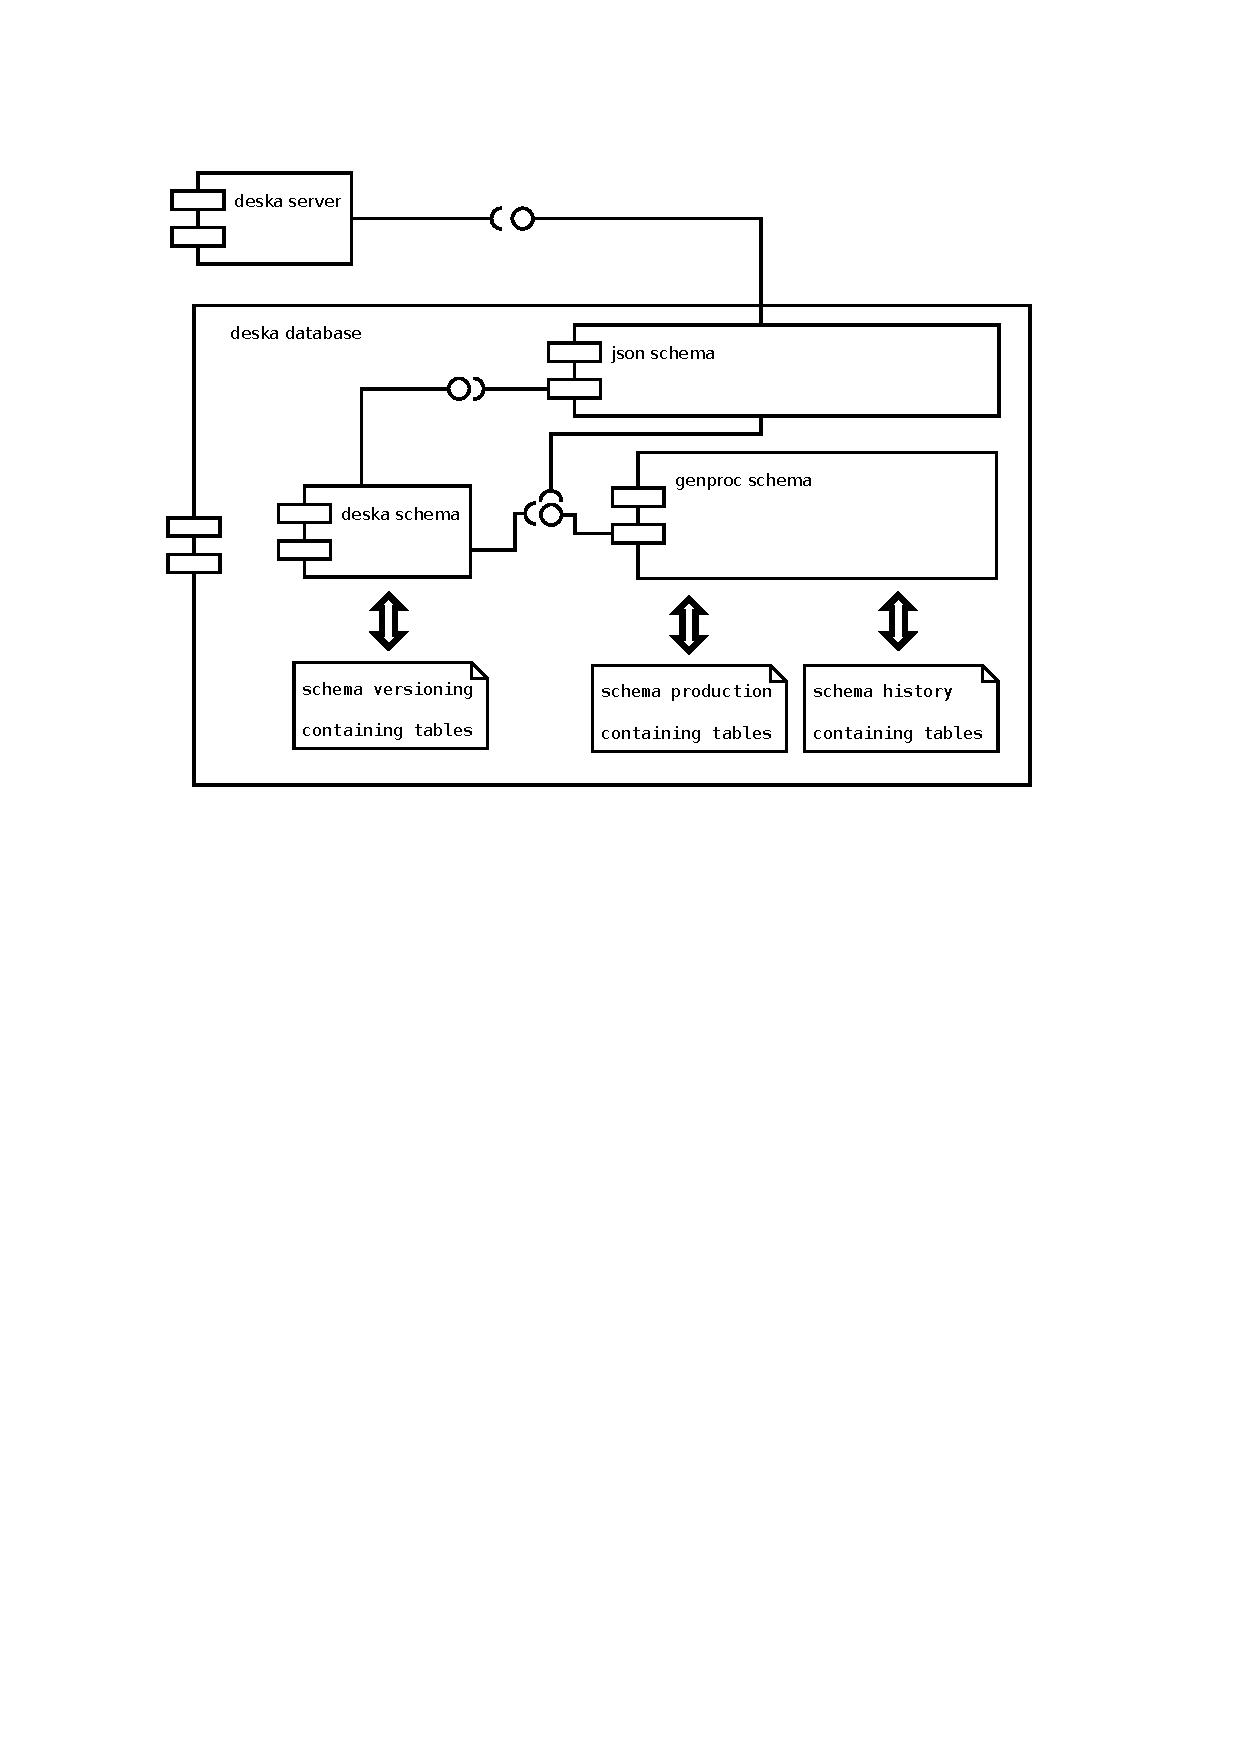
\includegraphics[trim=28mm 170mm 30mm 28mm]{img-deska-server-components.pdf}
	\caption{Deska server components}
\end{figure}

The philosophy of this desing is, that deska-server calls function in json schema (deska user is db role, for normal user, and it has rights only to run functions in schama json). Functions in json schema are using functions from deska schema (for work with versioning tables) or functions from genproc schema (for work with history and production tables).

\subsection{Filters}

\subsubsection{Function of filter}

Some functions in json schema have parametr filter. It is in json fomrat, see dbapi protocol for more info.
This filter is implemented in filter.py file in class filter. It support creation of WHERE part, that is added to select statement called from functions with filter parametr, and also JOIN part which is used in the same way.

As we said, some kind specific function is determined, for example hardware\_get\_version() (as data source for multipleObjectData function). There for some "SELECT [columns definition here] FROM hardware\_get\_version() AS hardware" is created. But if there is used some filter, we have to add WHERE part to this select. If the filter ask for some attribute of another kind, for example name of host which runs on the hardware, even JOIN part must be added. For it, there are Filter class methods getWhere and getJoin. 

Here it must be said, that you can join only kind (in fact it is some view on table, implemented as a function), which is in some relation with kind we operate with. The filter works with all relations and both directions presented in deska, but not transitively.

\subsubsection{Implementation}

The filters are created from two classes. Filter, which contains information about filter itself, parse the filter and creates
the JOIN and WHERE part of sql select statement. And Condition class, which stores information about each condition in filter, and provides
one sql part of WHERE part. It takes information from condition definition in filter parametr, and also from relation information provided
in generated.py file output of generators.

\subsection{Error handling}
Here we try to explain work with exception in deska database/ server. Postgre sql functions can RAISE exception with given message and sqlstate.
This sqlstate is like number of error. We use this to split posible exceptions into some category - exception types. Exception in database is
every unexpected or “bad” thing that occures. It can be run time error as well as contraint violation, or exception thrown explicitly by RAISE.

Psycopg2 used in deska-server to perform actions in db, has no good way to get sqlstate of exception, whích is used to determine exception type.
This is reason to catch maximum number of exception inside the database (in json schema part), so that exception type can be determined.

Functions in json schema catches all exceptions and transform it into json - see format of this execption in dbapi specification.
For this transformation DeskaException class is used. It has constructor, with Postgresql.dberr, which is structure that contains exception
message, and sqlstate. We use this information to determine exception type - class contains typeDict - dictionary {sqlstate: exceptionType}.
Finally this function has json method, which takes name on the function, in which error occures and creates exception in json format.

\end{document}
